% Figures used: fig0_architecture, fig3_forcing_cost.
\documentclass[conference]{IEEEtran}
\IEEEoverridecommandlockouts

\usepackage{cite}
\usepackage{amsmath,amssymb}
\usepackage{graphicx}
\usepackage{booktabs}
\usepackage{url}
\usepackage[hidelinks]{hyperref}
\graphicspath{{figures/}}
\setlength{\textfloatsep}{7pt plus 2pt minus 2pt}
\setlength{\dbltextfloatsep}{7pt plus 2pt minus 2pt}

\newcommand{\GI}{G\textsubscript{1}}
\newcommand{\GII}{G\textsubscript{2}}
\newcommand{\GIII}{G\textsubscript{3}}
\newcommand{\GIV}{G\textsubscript{4}}

\begin{document}

\title{Fail-Closed or Fail-Degraded? A Simulation Study \\of Forced Assurance
Loss in Contested Multi-Hop QKD Networks}

% Three affiliations do not fit side by side at this text width -- IEEEtran wraps to
% a second row and left-aligns it. The reference-mark form below is the class's own
% idiom for that case: it centres cleanly, keeps all three institutions, and is
% three lines shorter than the wrapped two-row layout.
\author{
\IEEEauthorblockN{Lakshya Jain\IEEEauthorrefmark{1},
Siddhi Arora\IEEEauthorrefmark{2},
Divya Mishra\IEEEauthorrefmark{3}}
\IEEEauthorblockA{
\IEEEauthorrefmark{1}\textit{Maharaja Agrasen Institute of Technology}, Delhi, India, 10jainlakshya@gmail.com\\
\IEEEauthorrefmark{2}\textit{Noida Institute of Engineering and Technology}, Greater Noida, India, Sid.arora1701@gmail.com\\
\IEEEauthorrefmark{3}\textit{G.L. Bajaj Institute of Technology and Management}, Greater Noida, India, divya\_rbl2@yahoo.com
}
}

\maketitle

\begin{abstract}
In multi-hop trusted-relay quantum key distribution (QKD), secret key is a
depletable per-link resource, since every hop of a relayed path consumes it. How a
network should behave when it runs short is unsettled: ITU-T Y.3803 permits
degradation, allowing a symmetric cipher to replace one-time-pad key relay, and
deployments follow it, whereas a recent layered design refuses, treating the
transition as a downgrade attack and failing closed. No study measures either
position against the other, to our knowledge. We quantify the trade-off, modelling a
nine-node tactical relay formation with per-link key reservoirs under an adversary
that raises the quantum bit error rate (QBER) until affected links abort key
generation. We introduce \emph{forced assurance loss}---the fraction of sessions
entitled to an information-theoretically secure key that are served without one---and
the \emph{downgrade-forcing cost}, the adversary budget required to induce it.
Suppressing links equal in number to the minimum edge cut forces the choice:
fail-closed operation loses availability, 0.812 to 0.304, while fail-degraded
operation holds it at 0.973 and instead forces 67.4\% of entitled traffic below an
ITS-delivered key, from a baseline of zero. The forcing cost needs both a capability
fixed by the abort threshold and a budget equal to the minimum edge cut; below the
capability threshold, extra link budget buys an adversary almost nothing. The
assurance-grade composition of served traffic therefore belongs in QKD resilience
reporting alongside key-supply continuity. Our simulator is checked against four
published measurements, reproducing two and failing two in the same direction, which
locates an under-parameterised accounting term.
\end{abstract}

\begin{IEEEkeywords}
Quantum key distribution, trusted-relay networks, key management, post-quantum
cryptography, graceful degradation, military communications.
\end{IEEEkeywords}

\section{Introduction}
A brigade in mountainous terrain reaches its rear area through a chain of relay
sites, carrying command circuits rekeyed every few minutes, imagery encrypted at
one-time-pad rates, and bulk delay-tolerant logistics. Suppose the network can no
longer supply quantum key for all of it. Refusing service shows the commander an
outage, which he can act on; holding the circuit up and rekeying the imagery link
with a computationally secure algorithm shows him nothing, and the loss stays
invisible until audit. Which failure is preferable is not settled.

Trusted-relay operation makes the question sharp. Beyond one quantum channel's
reach, keys extend hop by hop, each node re-encrypting the end-to-end key under its
neighbour key with a one-time pad and an ITS authenticator~\cite{salvail}. An
$n$-hop path therefore consumes key on \emph{every} one of its $n$ links, and at
free-space per-hop rates of order $10^{2}$\,bit/s the key supply binds, not the
existence of a quantum channel.

Standards, fielded key managers and layered designs resolve exhaustion in two
opposing ways. One permits degradation: a symmetric cipher may substitute for
unavailable one-time-pad key, provided the method is recorded~\cite{itu3803}.
Deployments behave this way~\cite{makris}, and both branches can be placed under
policy control, falling back to key derivation where policy allows and blocking the
host where it does not~\cite{tysowski}. The other treats the transition as an
attack surface and fails closed, tearing down the tunnel to prevent a
\emph{downgrade attack}~\cite{spooren}---one design stating that position
explicitly, so we treat it as an engineering stance rather than established
practice. The concern predates the mechanism: an adversary unable to steal quantum
keys may deny them instead, precisely to \emph{force} classical cryptography into
use~\cite{schartner}.

\textbf{The gap.} Neither branch has been measured: the fallback is specified in
design documents reporting no simulation or experiment~\cite{tysowski}, and we are
aware of no study quantifying what either branch costs, or what an adversary must
spend to force the choice. The modes hand the adversary different currencies---
refusal converts attack effort into visible outage, degradation into silent
assurance loss---so an operator choosing between them chooses blind. That the
architecture is prior art strengthens the case for measuring it: a mechanism
standards permit and deployments run is a more consequential target than an unused
design.

\textbf{Contributions.} (i) A threat-aware degradation model: pressure in absolute
QBER units, zero key past the security-abort threshold, and classical-channel
denial and QBER-invisible detector attacks as distinct states (\S\ref{sec:link}).
(ii) Two metrics---\emph{forced assurance loss}, defined on traffic \emph{entitled}
to ITS key, and the \emph{downgrade-forcing cost}---with a sensitivity analysis
separating the latter into capability and budget requirements (\S\ref{sec:head},
\S\ref{sec:sens}).
(iii) An analysis of key-aware routing under a fallback: when the availability
metric stops discriminating between policies, and why hop-multiplied cost penalises
key-aware paths, with paired intervals under common random numbers
(\S\ref{sec:routing}). (iv) A policy-space audit of an interpretable heuristic
against a searched policy under distribution shift (\S\ref{sec:audit}).
(v) A simulator checked against four published measurements, reproducing two and
failing two in the same direction, locating an under-parameterised accounting term
(\S\ref{sec:valid}).

\section{Related Work}
\begin{table}[t]
\caption{Dimensions addressed by representative trusted-relay QKD studies, in the
order the text discusses them.}
\label{tab:pos}
\centering\footnotesize
\setlength{\tabcolsep}{3.5pt}
\begin{tabular}{@{}lccccccc@{}}
\toprule
Work & MH & KS & TC & AD & SW & FB & FA\\
\midrule
Routing~\cite{vanduijn,johann,hao} & \checkmark & \checkmark & & & & & \\
\addlinespace[2pt]
Mehic \emph{et al.}~\cite{mehic} & \checkmark & \checkmark & \checkmark & $\circ$ & & & \\
Cao \emph{et al.}~\cite{cao} & \checkmark & \checkmark & $\circ$ & & & & \\
\addlinespace[2pt]
Tysowski \emph{et al.}~\cite{tysowski} & \checkmark & \checkmark & \checkmark & & & \checkmark & \\
Sanz \emph{et al.}~\cite{sanz} & \checkmark & & \checkmark & & & \checkmark & \\
Zhu~\cite{zhu} & $\circ$ & \checkmark & \checkmark & & & \checkmark & $\circ$\\
Makris \emph{et al.}~\cite{makris} & \checkmark & $\circ$ & & $\circ$ & & \checkmark & \\
Spooren \emph{et al.}~\cite{spooren} & \checkmark & & & $\circ$ & & $\dagger$ & \\
\addlinespace[2pt]
Li \emph{et al.}~\cite{li} & \checkmark & \checkmark & & \checkmark & & & \\
Ghorab \emph{et al.}~\cite{ghorab} & \checkmark & \checkmark & & \checkmark & \checkmark & & \\
Hafeez \emph{et al.}~\cite{hafeez} & \checkmark & \checkmark & & \checkmark & \checkmark & \checkmark & \\
\midrule
\textbf{This work} & \checkmark & \checkmark & \checkmark & \checkmark & \checkmark & \checkmark & \checkmark\\
\bottomrule
\end{tabular}
\begin{flushleft}\footnotesize
\emph{MH} multi-hop relay; \emph{KS} scarcity binding; \emph{TC} traffic classes;
\emph{AD} adversary modelled; \emph{SW} pressure swept; \emph{FB} fallback to
computationally secure key; \emph{FA} assurance loss on entitled traffic.
\checkmark~addressed; $\circ$~partial; blank~none; $\dagger$~specifies the transition
but fails closed.
\end{flushleft}
\end{table}

Trusted-relay QKD research follows four largely independent lines. The first asks
which path a request should take under key scarcity~\cite{vanduijn,johann,hao,cvitic};
the second adds priority classes and admission control~\cite{mehic}, coupling key
supply to an optical control plane~\cite{cao}. Both share one outcome model: a request obtains a path with
sufficient key on every hop, or it is blocked. Priority decides \emph{which}
requests receive quantum key, not \emph{what kind}, so neither can express service
at lower assurance.

The third line addresses exhaustion directly. Standards and key managers permit
substitution, provided it is recorded~\cite{itu3803,tysowski}; deployments
implement this~\cite{makris}, graded delivery has been specified with
controller-selected assurance tiers~\cite{sanz}. A
techno-economic study comes closest to costing it~\cite{zhu}, whereas a layered
QKD/post-quantum design treats the transition as an attack surface and fails
closed~\cite{spooren}. These are specifications and demonstrations: except
partly~\cite{zhu}, they report what the mechanism does, not what it costs,
and~\cite{tysowski} contains no simulation or measurement. The fourth models an
adversary explicitly---attack-radius minimisation~\cite{li}, zero-trust
relays~\cite{ghorab}, swept degradation for 6G~\cite{hafeez}---but keeps the
served-or-blocked outcome, so pressure converts only into outage and the
force-classical-crypto threat~\cite{schartner} is unrepresented.

Table~\ref{tab:pos} summarises these dimensions; studies are included if they model
key supply across more than one relay hop, and columns are the properties a
fail-mode comparison requires. The assurance-aware column is empty: the fraction of
traffic \emph{entitled} to ITS key served below that grade is unreported in any
study we could locate, \cite{zhu} being nearest but neither restricted to entitled
traffic nor swept. No prior work evaluates fail-closed against fail-degraded
operation, or quantifies what forcing the choice costs an adversary.

\section{System Model}
Since \emph{hybrid} denotes key-combiner composition secure if one component
survives~\cite{ietfhybrid}, a QKD$\rightarrow$post-quantum substitution is not
hybrid; we call it a labelled grade downgrade, and use \emph{assurance grade} rather
than ``security level'', which denotes key length here.

\begin{figure}[t]
\centering
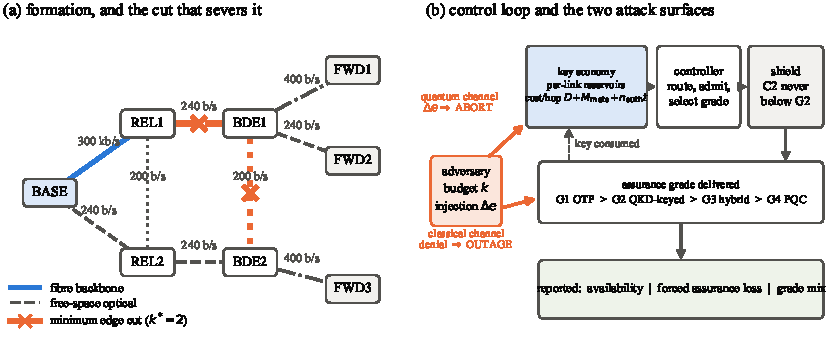
\includegraphics[width=\columnwidth]{fig0_architecture.pdf}
\caption{(a) The nine-node formation, per-link secret key rates and the minimum edge
cut. (b) The control loop; the adversary's two entry points are not equivalent
(\S\ref{sec:sens}).}
\label{fig:arch}
\end{figure}

We model (T1) a nine-node formation---rear node, two relays, two brigade nodes,
three forward posts; nine links, one fibre at 300\,kbit/s and eight free-space at
200--400\,bit/s (Fig.~\ref{fig:arch})---and (T2) a chain of depth $d$ with one longer lateral alternate. Each session is
routed, admitted and graded; a shield forbids command traffic below \GII; consumption
debits the per-link reservoirs.

Scarcity here is per link, not aggregate: the fibre link carries 300\,kbit/s against
2160\,bit/s across the eight free-space links, so consumption is 1.8\% of aggregate
capacity and most generated key overflows on the fibre. That key cannot move to where
it binds---$\approx$2900\,bit/s of demand must be met on the free-space hops alone,
exceeding their combined supply by 34\%. Stranded capacity one hop from the
bottleneck is the trusted-relay constraint, not an artefact of it.

Reservoirs use the QKDNetSim key-buffer semantics (READY/CHARGING/WARNING/EMPTY on
a threshold and a minimum), and key exceeding capacity is \emph{discarded}.
Capacity, threshold and minimum take that simulator's shipped SECOQC values:
$52\,428\,800$, $11\,324\,620$ and $1\,048\,576$ bits. The minimum doubles as an
\emph{authentication reserve}: SECOQC held a 2\,MiB floor to guarantee key for
classical-channel authentication~\cite{peev}. We could not locate a published
buffer capacity in vendor documentation or in the ETSI key-delivery
specification~\cite{etsi014}, so capacity is swept.

Sessions are served at four grades: \GI\ one-time pad (demand $=$ payload bits, per
Shannon~\cite{shannon}); \GII\ QKD-keyed symmetric (256\,bit,
ITS-\emph{delivered}); \GIII\ hybrid QKD\,$\oplus$\,ML-KEM-768 (128\,bit plus KEM,
via an approved domain-separated combiner); \GIV\ ML-KEM-768 only. Each class
carries an \emph{authorised floor}; unmet, the controller blocks
(\textsc{fail\_closed}) or serves below it and records an auditable violation
(\textsc{fail\_degraded}).

\subsection{Link model and adversary}\label{sec:link}
A two-state model giving a degraded link a fixed fraction of nominal rate is
indefensible under attack: an adversary raises noise above the security threshold,
and any perturbation sufficient for that halts key generation~\cite{alleaume}. We
use four states: \textsc{nominal} ($R_0$);
\textsc{degraded} ($R_0\rho(e)$); \textsc{abort} ($0$, for
$e\ge e_{\mathrm{abort}}$); \textsc{outage} ($0$; cut, LOS loss, \emph{or
classical-channel denial}), with
\begin{equation}
\rho(e)=\left[\frac{\max\!\left(0,\,1-fH_2(e)-H_2(e)\right)}
{1-fH_2(e_0)-H_2(e_0)}\right]^{\gamma},
\end{equation}
$f=1.16$ and $e_0=0.03$~\cite{sasaki}. We report $\gamma=1$ (asymptotic BB84,
following~\cite{ma}) and $\gamma=3.4$, calibrated to the only measured
degraded-link datapoint we found, a misaligned entanglement link delivering
0.25\,kbps at QBER 5--7\% against 2--3\,kbps nominal~\cite{sasaki}. These give 50\%
and 10\% at QBER 6\%; \textbf{we publish the disagreement as a sensitivity rather
than resolve it}. $e_{\mathrm{abort}}=0.075$ is an engineering value, the
distillation engine of~\cite{sasaki} supplying coding rates only below 3.5, 5.5 and
7.5\%; 0.11 is a sensitivity. Realistic error correction \emph{lowers} the ITS zero
from 11.0\% to 9.9\% at $f=1.16$.

Two failure modes bypass QBER and are separate states: classical post-processing
denial leaves the quantum channel pristine but halts key production~\cite{mehic},
and detector blinding by tailored bright illumination makes it possible to
``tracelessly acquire the full secret key''~\cite{lydersen}, so that attack is
invisible to any QBER-driven model including ours.

The adversary attacks availability to force a downgrade~\cite{schartner}, selecting
$k$ links and injecting excess QBER $\Delta e$; absolute QBER units make the
pressure checkable. Targeting is greedy by edge betweenness or \emph{minimum edge
cut}, the worst case.

\subsection{Key accounting and traffic}\label{sec:acct}
Relaying $D$ bits of key across one hop costs
$D+M_{\mathrm{meta}}+n_{\mathrm{auth}}t$, with metadata 240\,bit (Y.3803 relays a
\emph{key file}, not a bare key) and tag $t=127$\,bit~\cite{walenta}.
Wegman--Carter authentication is charged per message and grows only
\emph{logarithmically} in message length~\cite{fung}, so overhead depends on block
size: 2.93 times the delivered key at $D=256$, 1.000 at $D=1$\,Mbit. Zeroing the
authentication terms recovers the bare $D{\cdot}n$ law of the routing literature,
which we ablate.

The count $n_{\mathrm{auth}}$ of authenticated messages per key delivery is the one
term we could not ground in a specification. We set it to 2, mutual authentication
consuming two one-time keys per round. \S\ref{sec:valid} shows this is a lower bound
rather than a measurement---published relay overhead implies $\approx7$ per relay
hop, an application-level tunnel $\approx40$---so we sweep it and re-check the
headline, reporting at 2 as the optimistic end. The choice is not load-bearing,
for an arithmetic reason: one-time-pad ISR sessions contribute 2880 of the
2897\,bit/s of payload demand, against which authentication is a few hundred bits
per hop, so raising $n_{\mathrm{auth}}$ to the calibrated 7 costs 6.3\% more key and
to 40 costs 47.5\%. Absolute expenditure therefore scales with $n_{\mathrm{auth}}$;
the policy \emph{differences} of \S\ref{sec:routing} do not, being differences of a
common additive term.

The accounting carries some conclusions and not others. It decides which grades are
affordable---the \GI\ floor result of \S\ref{sec:head} is an accounting result---and
sets key expenditure and the \S\ref{sec:routing} comparison. It does not set the
availability headline, which is cut-limited: once min-cut links abort, no accounting
term restores a quantum path, so the \S\ref{sec:sens} insensitivity is expected
rather than evidence of idle accounting.

Demands come from measured deployments. C2: 2048\,bit, floor \GII, 5\,s,
$\lambda=0.05$\,s$^{-1}$ (256\,bit/min per encryptor, the modal deployed
unit~\cite{stucki}). ISR: 144\,000\,bit, floor \GI, 30\,s,
$\lambda=0.02$\,s$^{-1}$, a 60\,s session of the 2.4\,kbps one-time-pad voice run
31 months on a 46-node metro network~\cite{chen}. LOG: 320\,000\,bit,
floor \GIII, 120\,s, $\lambda=0.03$\,s$^{-1}$, from the same network's measured
320\,kbps file transfer.

\section{Experimental Setup}\label{sec:setup}
Discrete-event simulation, 1\,s resolution, 24\,h horizon, first 12\,h discarded.
The warm-up is itself a finding: from full reservoirs, free-space stores take
$\sim$12\,h to fall to the authentication reserve, so a 4\,h run leaves them at
59\% of capacity and measures the initial fill, not the key economy. \emph{Common
random numbers} give every policy identical arrival streams and channel
realisations per seed, so comparisons are paired, with paired bootstrap intervals
(20\,000 resamples). Twelve seeds for main comparisons, six for sweeps.

\subsection{Validation}\label{sec:valid}
Cross-validation against an established quantum-network simulator was unavailable:
SeQUeNCe, QuISP and NetSquid model point-to-point or entanglement-distribution physics
with no trusted-relay key pool, and \emph{a key-economy simulator cannot be validated
against tools that do not model a key economy}. QKDNetSim is the sole on-target
candidate and we adopt its buffer semantics verbatim, so our reservoir is citable
rather than invented; but its admission control is absent---one of the two mechanisms
compared here---and QKDNetSim+ reports nodes mishandling key material and a
malfunctioning crypto handler~\cite{qkdnetsimplus}, in the layer a cross-validation
would exercise. What can be checked externally is therefore
limited to three properties: the accounting arithmetic, supply against
field-measured demand, and key-delivery conformance. Policy behaviour cannot be,
because no deployment publishes the assurance-grade composition of its served
traffic---the quantity this paper introduces---so the limitation follows from the
metric being new, not from the method.

A 43-check gate covering key conservation, reservoir bounds and transitions, the rate
cliff and the degenerate cases in both fail modes must pass before any result is
reported. Beyond it we compare against four published measurements from three
deployments. \textbf{V1} reproduces the SECOQC rerouting experiment, where an
8192\,bit/s one-time-pad application drained 3.5\,MiB of a 5.5\,MiB store in about an
hour, to 3584\,s against a 3584\,s reference---internal consistency rather than
independent validation, the reference coming from the same accounting the model
applies. \textbf{V4} checks the one-time-pad demand law untuned: eleven bidirectional
2.4\,kbps voice pairs need 52.8\,kbps, and the model admits 1.2--12.6 pairs against
the 6--60.5\,kbps measured on that network, so the check bounds the demand law to an
order of magnitude rather than pinning it.

\textbf{V2 and V3 both fail, and the same way.} Cambridge distributed 1000 global
keys for about 180\,kbyte of link key~\cite{dynes}, $3.69\times$ the $\sim$400-bit
key delivered, against our $2.23\times$; SECOQC's tunnel spent 5824\,bit per rekey round of which
only 512\,bit was cipher key---91.2\% authentication---against our 65.9\%. Solving
each for authenticated messages per key delivery gives $n_{\rm auth}\approx7$ for a
relay hop and $\approx40$ for an application tunnel, against the 2 assumed. \textbf{Our $n_{\rm auth}=2$ is
a lower bound, not a measurement, and our per-hop cost is correspondingly
optimistic.} That fixes the \emph{direction} of the bias, which a reader needs; it
strengthens \S\ref{sec:acct}, since calibrating to Cambridge grows the bare
$D{\cdot}n$ understatement from 2.93$\times$ to 5.41$\times$ at 256-bit blocks; and
it forced the \S\ref{sec:sens} re-check, which the headline survives.

\section{Results}
\subsection{The fail-mode exchange rate}\label{sec:head}
\begin{table}[t]
\caption{Availability, floor violations and forced assurance loss versus adversary
budget (12 seeds, key-aware routing, $\Delta e=0.05$, betweenness targeting).
\emph{Viol.}: served below the class's authorised grade, possibly still ITS.
\emph{Forced}: \emph{entitled} to ITS key, served without. SD $\le0.012$.}
\label{tab:head}
\centering\footnotesize
\begin{tabular}{@{}llrrrrr@{}}
\toprule
Mode & $k$ & Avail. & \GII & \GIV & Viol. & Forced\\
\midrule
\textsc{closed} & 0 & 0.8124 & 0.590 & 0.000 & 0.000 & \textbf{0.000}\\
\textsc{closed} & 1 & 0.8264 & 0.564 & 0.000 & 0.000 & \textbf{0.000}\\
\textsc{closed} & 2 & \textbf{0.3039} & 0.508 & 0.000 & 0.000 & \textbf{0.000}\\
\textsc{closed} & 5 & \textbf{0.0000} & --- & --- & --- & ---\\
\textsc{degr.}  & 0 & 0.9733 & 0.659 & 0.000 & 0.166 & \textbf{0.000}\\
\textsc{degr.}  & 1 & 0.9733 & 0.607 & 0.029 & 0.157 & 0.029\\
\textsc{degr.}  & 2 & 0.9733 & 0.174 & \textbf{0.675} & 0.690 & \textbf{0.674}\\
\textsc{degr.}  & 5 & 0.9733 & 0.000 & \textbf{1.000} & 1.000 & \textbf{1.000}\\
\bottomrule
\end{tabular}
\end{table}

The transition is a cliff (Table~\ref{tab:head}). Suppressing 2 of 9 links
collapses fail-closed availability from 0.812 to 0.304, while fail-degraded
operation holds availability at 0.973 and converts the same pressure into 67.4\%
forced assurance loss, post-quantum-only service rising from 2.9\% to 67.5\%. At
$k=5$ both endpoints are total: complete denial, or complete assurance loss at
undiminished availability.

One row is non-monotone and the mechanism matters: at $k=1$ fail-closed availability
\emph{rises} to 0.826 (paired $+0.0140$, CI $[+0.0082,+0.0193]$). Aborting one link
removes a long path from the router's choice set, so mean path length falls 3.086 to
3.029 hops, expenditure falls 6.8\%, and the freed key funds the starved one-time-pad
class, whose service nearly doubles from 0.167 to 0.321 while command and logistics
give up 2.7 and 1.1 points. A weak attack acts as inadvertent admission
control---the hop multiplier of \S\ref{sec:routing} from the other side---so $k=0$ is
the correct reference for the collapse.

The value 2 is not peculiar to our formation: it is the \emph{minimum edge cut}
from rear node to forward posts, and severing a cut removes every quantum-viable
path by definition. We therefore treat $k^\ast=$ min-cut as an observation, not a
finding, and use it as a check on the adversary search, which recovers the optimum
unaided. What is \emph{not} definitional is the cost of reaching that cut without
knowing the graph, which \S\ref{sec:cost} measures.

\textbf{Two distinct losses, and only one belongs to the adversary.} Forced
assurance loss is 0.000 at $k=0$ in both modes: unattacked, every entitled session
receives an ITS-delivered key, so every point at $k>0$ is attributable to the attack
with no baseline artefact to subtract. Floor violations are not zero there. They
stand at 0.166, because ISR traffic reaches its \GI\ one-time-pad floor in only 555
of 3349 sessions and is otherwise served at \GII---below its authorised grade, but
still ITS-delivered. A one-time-pad floor for a 144\,kbit session is not fundable at
these rates, demand exceeding per-hop supply by three orders of magnitude, so a
policy written at that floor is unimplementable before any adversary acts.

\subsection{Three negative results for key-aware routing}\label{sec:routing}
All three policies are compared at $k=0$ over twelve common seeds; forced assurance
loss is 0.000 in every one, no adversary being present.

\textbf{(1) The service metric becomes degenerate.} A post-quantum fallback
succeeds on every session for which a classical path exists, in every seed, so
availability becomes a property of connectivity rather than of key-awareness. All
three policies hold availability at 0.9733, and the paired difference between them is
consequently $0.0000$ with a 95\% CI of \emph{zero width}---an exact result, not an
absent one. In this model the metric the
key-aware-routing literature reports stops responding to the property it is taken
to measure. Routing still moves key expenditure significantly: key-aware routing
spends $+27.0$\,Mbit, CI $[+25.3,+28.9]$, and class-aware floors $-38.1$\,Mbit, CI
$[-40.5,-35.7]$, against shortest path.

\textbf{(2) Under fail-closed operation the hop multiplier penalises key-aware
path selection.} Our router loses 2.7 points of availability to shortest path
(0.8124 against 0.8392; $-0.0268$, CI $[-0.0293,-0.0242]$), because it selects longer paths
(3.086 against 3.062 hops) and every extra hop consumes key on an \emph{additional}
link, raising expenditure 6.0\% and starving later sessions. Sweeping the hop
penalty over four orders of magnitude does not repair it. We did not reimplement a
published key-aware algorithm, so we scope this to the mechanism and to our own
implementation: hop-multiplied cost with authentication charged penalises longer
paths under binding scarcity and fail-closed semantics. Where prior work reports
25--40\% improvements~\cite{cvitic} it measures blocking under different scarcity
and without a fallback.

\textbf{(3) Reservation floors are an admission decision, not a graded control.}
Class-aware floors appear to buy assurance with availability,
$0.839\rightarrow0.509$ against served sessions carrying no ITS-delivered key,
$0.357\rightarrow0.000$, but the mechanism is denial: logistics traffic, the one class authorised below ITS, drops
from 0.988 served to 0.000 because its floor sits above the level at which
higher-priority draws pin the reservoir. Nor is it tunable---sweeping the floor
scale over two orders of magnitude switches between $(0.51, 0.000)$ with logistics
denied and $(0.81, 0.362)$ with logistics served, with no useful intermediate,
because a demand-saturated link sits within a few percent of the authentication
reserve, so a floor is either inert or absolute. Per-class floors are an admission
decision rather than a graded control---the \GI\ unimplementability of
\S\ref{sec:head} by another route.

\subsection{Downgrade-forcing cost versus depth}\label{sec:cost}
\begin{figure}[t]
\centering
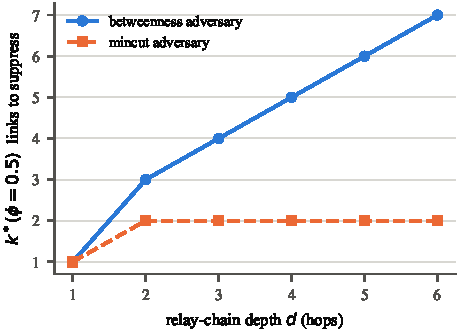
\includegraphics[width=\columnwidth]{fig3_forcing_cost.pdf}
\caption{Forcing cost $k^\ast(\phi{=}0.5)$ against relay-chain depth for a greedy
centrality-guided and an optimal minimum-cut adversary.}
\label{fig:cost}
\end{figure}

This result concerns the adversary model, not the graph. On \emph{forced} degradation,
nominal loss is 0.000 at every depth, so every point is attributable to the attack. A
greedy centrality-guided adversary needs $k^\ast = d+1$ links beyond $d=1$, linear in
depth, because it exhausts the already-severed primary path before touching the
alternate; a minimum-cut adversary needs \textbf{two at every depth beyond $d=1$}
(Fig.~\ref{fig:cost}). The gap is the finding: \emph{which adversary a study reports
determines the resilience it claims, by a factor growing with relay
depth}---$3.5\times$ at $d=6$. Sweeping only a greedy adversary overstates resilience,
and relay depth buys no protection against a competent one.

\subsection{Sensitivity and operating envelope}\label{sec:sens}
The five-fold ambiguity in $\gamma$ barely matters: fail-closed availability at
$k=2$ is 0.302 at \emph{both} values when $e_{\mathrm{abort}}=0.075$. The abort
threshold decides the outcome instead, and its location is arithmetic on our
definitions rather than a discovery: since $\rho(e)=0$ for
$e \ge e_{\mathrm{abort}}$, a link at nominal $e_0$ aborts when
$\Delta e \ge e_{\mathrm{abort}}-e_0$---0.045 at $e_{\mathrm{abort}}=0.075$, 0.08 at
0.11. The sweep turns there, and confirming a definition is not a finding.

\begin{table}[t]
\caption{Budget does not substitute for capability. Fail-closed availability at
sub-threshold injection ($e_{\mathrm{abort}}=0.075$, so the capability threshold is
$\Delta e = 0.045$), across a five-fold range in link budget; 6 seeds. Forced
assurance loss stays $\le0.0002$ in every cell. For contrast, one step past the
threshold at $\Delta e=0.05$ gives availability 0.302 and forced loss 0.677.}
\label{tab:envelope}
\centering\footnotesize
\setlength{\tabcolsep}{4pt}
\begin{tabular}{@{}lrrrrrr@{}}
\toprule
$\Delta e$ & $k{=}1$ & $k{=}2$ & $k{=}3$ & $k{=}4$ & $k{=}5$ & span\\
\midrule
0.01 & 0.8102 & 0.8055 & 0.8055 & 0.8055 & 0.8055 & 0.0047\\
0.02 & 0.8102 & 0.8014 & 0.8014 & 0.8014 & 0.8014 & 0.0087\\
0.03 & 0.8102 & 0.7982 & 0.7982 & 0.7982 & 0.7982 & 0.0120\\
0.04 & 0.8102 & 0.7956 & 0.7956 & 0.7956 & 0.7956 & 0.0146\\
\bottomrule
\end{tabular}
\end{table}

What the sweep does establish requires the budget varied, not held at the cut.
Table~\ref{tab:envelope} sweeps $k \in \{1,\dots,5\}$ at each sub-threshold
injection: availability moves by at most 0.015 and forced assurance loss stays below
0.0002. Budgets of two and above coincide to four decimal places, because the links a
centrality-guided adversary picks beyond the cut have reservoir slack, so degrading
them does not bind. An adversary that cannot reach the capability threshold therefore
gains almost nothing from a five-fold larger budget: the two requirements do not
substitute, and the forcing cost is bounded below by each independently. That is a
property of steady-state slack rather than of the step function, and it tells a
defender which quantity an investment moves: raising $e_{\mathrm{abort}}$ from
0.075 to 0.11 raises the required injection by \textbf{78\%}, and it is set by
reconciliation efficiency, not key rate.

\textbf{The fallback needs the classical channel.} Fail-degraded availability is
invariant under QBER injection because a link in \textsc{abort} still carries a
pristine classical channel, and ML-KEM needs only that. Under classical-channel
denial availability falls from 0.970 to \textbf{0.313}---1.6 points above
fail-closed's 0.296---and forced loss is zero because severed posts are blocked
outright rather than downgraded. \emph{The entire advantage of degrading gracefully
is conditional on the classical channel surviving.}

\textbf{The headline survives the authentication recalibration.} Sweeping
$n_{\mathrm{auth}} \in \{2,7,20,40\}$---a 7.4-fold range in per-hop cost at a
256-bit block---moves fail-closed availability at $k=2$ only from 0.302 to 0.281
and leaves fail-degraded forced loss at 0.678, for the cut-limited reason given in
\S\ref{sec:acct}.

\subsection{Policy-space audit}\label{sec:audit}
Grade selection under scarcity suits reinforcement learning, but a policy posting a
better number in our own simulator would be unfalsifiable, so we instead asked how
much headroom the heuristic leaves: we search a 12-cell state$\rightarrow$grade table
by the cross-entropy method with full rollouts, behind a shield masking any action
that places command traffic below \GII. The heuristic reaches 104.8\% of the best
\emph{shielded} searched policy and wins all seven out-of-distribution conditions,
though the two do not order componentwise---the searched policy wins availability,
0.9726 against 0.8123, and pays 39.5\% floor violations. Writing
$J=\text{avail}-\lambda\cdot\text{viol}+w\cdot\text{ITS}$, the heuristic wins exactly
when $\lambda>0.370$ at $w=0.5$ (0.406 at $w=0$, 0.264 at $w=2$); that price, not a
winner, is the useful output, and locating it required the search. Two mechanisms
transfer beyond QKD. The searched policy \emph{beat} the heuristic on its 6\,h
training horizon ($J$ 1.4591 against 1.2978) and lost at 24\,h, because reservoirs
take $\sim$12\,h to drain to the authentication reserve (\S\ref{sec:setup}) and
training sampled only the key-abundant regime: a learned controller sharing a
depletable resource needs a horizon spanning the depletion timescale, and the failure
is invisible from training curves. And removing the shield scored highest of all,
cutting key consumption from 464 to 42\,Mbit while keeping every session on
ITS-\emph{delivered} key, by serving one-time-pad-entitled ISR traffic at \GII---so a
shield written for one class is circumvented through the classes it omits, and floors
must be specified \emph{and} priced per class.

\section{Discussion and Limitations}
Choosing between refusing and degrading chooses which resource the adversary takes,
at a steep exchange rate. Limitations: per-link key rates are parameterised inputs,
not simulated photonics; the two degradation calibrations disagree five-fold and we
report both; relay nodes are trusted, compromise modelled only as availability loss;
detector blinding raises no QBER and is invisible here by construction; the headline
rests on one formation, with one chain family in \S\ref{sec:cost}; unmeasured
parameters are swept rather than assumed; the policy audit used a modest search
budget; and class-aware floors are reported as the admission decision they turn out
to be, no floor scale we swept producing a useful intermediate. Next steps:
QKDNetSim cross-validation, a second headline topology, a reimplemented published
router.

Also open: a grade attribute on the delivered key so consumers can enforce policy,
absent from the current REST interface~\cite{etsi014}; and spatially correlated
free-space outage, which every model we found treats as independent.

\section{Conclusion}
Standards permit fallback to weaker key supply; a layered post-quantum design
forbids it as a downgrade attack. We measured the trade-off. Suppressing links equal to the minimum edge
cut either collapses availability from 0.812 to 0.304, or holds it at 0.973 while
forcing 67.4\% of entitled traffic below ITS protection from a baseline of zero. The
forcing cost requires both a per-link capability and a budget, which do not
substitute. A post-quantum fallback also makes the key-aware-routing service metric
degenerate, hop-multiplied cost costs key-aware paths 2.7 availability points under
fail-closed semantics, and degrading gracefully is conditional on the classical
channel surviving.
We argue that the assurance-grade composition of \emph{served} traffic belongs in
QKD resilience reporting alongside key-supply continuity.

\section*{Reproducibility and Acknowledgements}
The simulator, all configurations, the 43-check validation gate and every figure and
table script are available from the authors and will be deposited publicly on
acceptance; the full set runs in $\sim$30\,min on eight CPU cores, no GPU. ITU-T and
ETSI products are not redistributed; a download script is provided. The authors used a
large language model as a coding and drafting assistant for the simulator, figures
and manuscript. All modelling decisions, parameter provenance, experimental design
and claims are the authors', and every reported number was produced by the released
code.

\begin{thebibliography}{00}
\bibitem{salvail} L. Salvail \emph{et al.}, ``Security of trusted repeater QKD networks,'' \emph{J. Comput. Secur.}, vol.~19, pp.~61--106, 2011.
\bibitem{itu3803} ITU-T Rec.~Y.3803, \emph{QKD networks---Key management}, 12/2020, cl.~8.2.3, 8.2.5.
\bibitem{makris} A. Makris \emph{et al.}, ``Field demonstration of a fully managed L1-encrypted 3-node network with hybrid relayed-QKD,'' in \emph{Proc. ECOC}, 2024.
\bibitem{tysowski} P.~K. Tysowski \emph{et al.}, ``The engineering of a scalable multi-site communications system utilizing quantum key distribution (QKD),'' \emph{Quantum Sci. Technol.}, vol.~3, no.~2, 024001, 2018, doi:10.1088/2058-9565/aa9a5d.
\bibitem{spooren} P. Spooren \emph{et al.}, ``PQC-enhanced QKD networks: a layered approach,'' in \emph{IEEE QCNC}, 2026.
\bibitem{schartner} P. Schartner and S. Rass, ``Quantum key distribution and denial-of-service: using strengthened classical cryptography as a fallback option,'' in \emph{Proc. Int. Computer Symp.}, 2010, pp.~131--136.
\bibitem{vanduijn} T. van Duijn \emph{et al.}, ``Routing strategies for QKD networks based on trusted relay nodes,'' in \emph{Proc. ONDM}, 2024.
\bibitem{johann} T. Johann \emph{et al.}, ``Comparison and optimization of routing methods for meshed QKD networks using trusted nodes,'' \emph{J. Opt. Commun. Netw.}, vol.~16, no.~3, pp.~382--391, 2024.
\bibitem{hao} Y. Hao \emph{et al.}, ``Q-learning for resource-aware and adaptive routing in trusted-relay QKD network,'' \emph{Photonics}, vol.~12, no.~10, 969, 2025.
\bibitem{mehic} M. Mehic \emph{et al.}, ``A novel approach to QoS provisioning in trusted relay QKD networks,'' \emph{IEEE/ACM Trans. Netw.}, vol.~28, 2020.
\bibitem{cao} Y. Cao \emph{et al.}, ``Key on demand for software-defined optical networks secured by QKD,'' \emph{Opt. Express}, vol.~25, no.~22, 2017.
\bibitem{sanz} A. Sanz \emph{et al.}, ``Extending quantum-safe communications to real-world networks,'' arXiv:2511.22416, 2025.
\bibitem{zhu} Z. Zhu, ``Techno-economic feasibility analysis of QKD for power-system communications,'' arXiv:2510.15248, 2025.
\bibitem{li} M. Li \emph{et al.}, ``Routing and wavelength assignment with minimal attack radius for QKD networks,'' arXiv:2508.10613, 2025.
\bibitem{ghorab} A. Ghorab \emph{et al.}, ``A QKD routing scheme for a zero-trust QKD network system,'' \emph{Big Data Cogn. Comput.}, vol.~9, no.~4, 76, 2025.
\bibitem{hafeez} M. Hafeez \emph{et al.}, ``Quantum-secured routing in drone communication for 6G-enabled smart mobility,'' \emph{Sci. Rep.}, 2026.
\bibitem{cvitic} I. Cviti\'c, D. Perakovi\'c, and A.~N. Pinto, ``Overview of routing approaches in QKD networks,'' arXiv:2511.15465, 2025.
\bibitem{ietfhybrid} IETF TLS WG, \emph{Hybrid key exchange in TLS 1.3}, draft-ietf-tls-hybrid-design, \S1.2.
\bibitem{peev} M. Peev \emph{et al.}, ``The SECOQC QKD network in Vienna,'' \emph{New J. Phys.}, 11, 075001, 2009.
\bibitem{etsi014} ETSI GS QKD 014 V1.1.1, \emph{Protocol and data format of REST-based key delivery API}.
\bibitem{shannon} C.~E. Shannon, ``Communication theory of secrecy systems,'' \emph{Bell Syst. Tech. J.}, vol.~28, no.~4, pp.~656--715, 1949.
\bibitem{alleaume} R. All\'eaume \emph{et al.}, ``Using QKD for cryptographic purposes: a survey,'' \emph{Theor. Comput. Sci.}, vol.~560, pp.~62--81, 2014.
\bibitem{sasaki} M. Sasaki \emph{et al.}, ``Field test of QKD in the Tokyo QKD Network,'' \emph{Opt. Express}, vol.~19, no.~11, pp.~10387--10409, 2011.
\bibitem{ma} X. Ma \emph{et al.}, ``Practical decoy state for QKD,'' \emph{Phys. Rev. A}, vol.~72, 012326, 2005.
\bibitem{lydersen} L. Lydersen \emph{et al.}, ``Hacking commercial quantum cryptography systems by tailored bright illumination,'' \emph{Nature Photonics}, vol.~4, no.~10, pp.~686--689, 2010, doi:10.1038/nphoton.2010.214.
\bibitem{walenta} N. Walenta \emph{et al.}, ``A fast and versatile QKD system with hardware key distillation and wavelength multiplexing,'' arXiv:1309.2583.
\bibitem{fung} C.-H.~F. Fung \emph{et al.}, ``Practical issues in QKD postprocessing,'' arXiv:0910.0312.
\bibitem{stucki} D. Stucki \emph{et al.}, ``Long-term performance of the SwissQuantum QKD network in a field environment,'' \emph{New J. Phys.}, vol.~13, 123001, 2011.
\bibitem{chen} T.-Y. Chen \emph{et al.}, ``Implementation of a 46-node quantum metropolitan area network,'' \emph{npj Quantum Information}, vol.~7, 134, 2021, doi:10.1038/s41534-021-00474-3.
\bibitem{qkdnetsimplus} M. Mehic \emph{et al.}, ``QKDNetSim+: improvement of the quantum network simulator for NS-3,'' arXiv:2402.10822, 2024.
\bibitem{dynes} J.~F. Dynes \emph{et al.}, ``Cambridge quantum network,'' \emph{npj Quantum Inf.}, vol.~5, 101, 2019.
\end{thebibliography}
\end{document}
